% CS 418: Intro to Data Science — Worksheet 26 (26-week13-day2)
% Week 13, Wednesday 2026-11-18
% Compile with: latexmk -pdf worksheet.tex

\documentclass[11pt]{article}

% ── Packages ──────────────────────────────────────────────────────────────────
\usepackage[margin=0.65in, headheight=14pt]{geometry}
\usepackage{amsmath, amssymb}
\usepackage{ragged2e}
% Never break a word across lines, including at hyphens ("Sans-Serif").
\hyphenpenalty=10000
\exhyphenpenalty=10000
\usepackage{enumitem}
\usepackage{booktabs}
\usepackage{graphicx}
\usepackage{hyperref}
\usepackage{xcolor}
\usepackage{fancyhdr}
\usepackage{mdframed}
\usepackage{array}
\usepackage{multicol}

% ── Page style ────────────────────────────────────────────────────────────────
\pagestyle{fancy}
\fancyhf{}
\lhead{\textbf{CS 418: Intro to Data Science}}
\rhead{UIC, Fall 2026}
\cfoot{\thepage}
\renewcommand{\headrulewidth}{1pt}
\setlength{\headheight}{12pt}
\setlength{\headsep}{0.4cm}

% ── Hyperlinks ────────────────────────────────────────────────────────────────
\hypersetup{colorlinks=false, hidelinks}

% ══════════════════════════════════════════════════════════════════════════════
\begin{document}
\RaggedRight

% ── Title block: topic left, info box right ───────────────────────────────────
\noindent
\begin{minipage}[t]{0.55\textwidth}
  \vspace{0pt}
  {\LARGE \textbf{Worksheet \#\,26}} \\[0.18em]
  {\large \textit{Week 13, Day 2: Data visualizations ``in the wild''}} \\[0.18em]
  {\small Asynchronous (Canvas discussion)}
\end{minipage}
\hfill
\begin{minipage}[t]{0.40\textwidth}
  \vspace{0pt}
  \small
  Name: \underline{\hspace{4.5cm}} \\[0.35em]
  NetID: \underline{\hspace{4.3cm}} \\[0.35em]
  Date: \underline{\hspace{4.4cm}} \\
\end{minipage}

\vspace{0.5em}
\noindent\rule{\linewidth}{0.6pt}
\vspace{0.3em}

Choose a data visualization that you have encountered recently - it can be from a news article, television, TikTok, Instagram, Snapchat, or some other media channel. For this worksheet, you will:

\begin{enumerate}[itemsep=0.1em, topsep=0.3em]
  \item Choose a visualization
  \item Write a brief ``review'' of the visualization you chose
  \item Review another visualization in the thread
\end{enumerate}

\vspace{0.3em}
For your ``reviews,'' include at least two strengths of the visualization (i.e.\ two things it communicates effectively), and at least two aspects you might change (these can be improvements or just ``remixes'').

\vspace{0.3em}
If you don't have a visualization in mind and you want to explore options, you might peruse the following websites:

\begin{itemize}[itemsep=0.1em, topsep=0.3em]
  \item The Pudding: \url{https://pudding.cool}
  \item r/DataIsBeautiful: \url{https://www.reddit.com/r/dataisbeautiful/}
  \item Our World in Data: \url{https://ourworldindata.org}
  \item Information is Beautiful: \url{https://informationisbeautiful.net}
  \item Pew Research Center: \url{https://www.pewresearch.org}
  \item ProPublica: \url{https://www.propublica.org}
  \item The Guardian datablog: \url{https://www.theguardian.com/news/datablog}
  \item FlowingData: \url{https://flowingdata.com}
\end{itemize}

\vspace{2.2em}
Please use the squishy fleshy bloody organ inside your skull for this exercise, and resist the urge to have an AI/LLM write the review.

\vspace{2.2em}
It's near the end of the semester and we've all seen enough slop at this point.

\vspace{2.2em}
Your classmates will appreciate seeing an interesting visualization and getting to read real, meaningful, human language about it.

\vspace{2.2em}
Your review doesn't need to be eloquent, it just needs to be your own words!

\vspace{2.2em}
If you have any questions, please email me (\href{mailto:jxb@uic.edu}{jxb@uic.edu})

\newpage

% ── Example review ───────────────────────────────────────────────────────────
% flock-cameras.png is multiple_urban_areas_have_thousands_of_flock_cameras.png from the Pew short read linked below.
\noindent{\large\textbf{Example Review}}\\[0.1em]
\noindent\textit{by Prof.\ Bandy}

\begin{center}
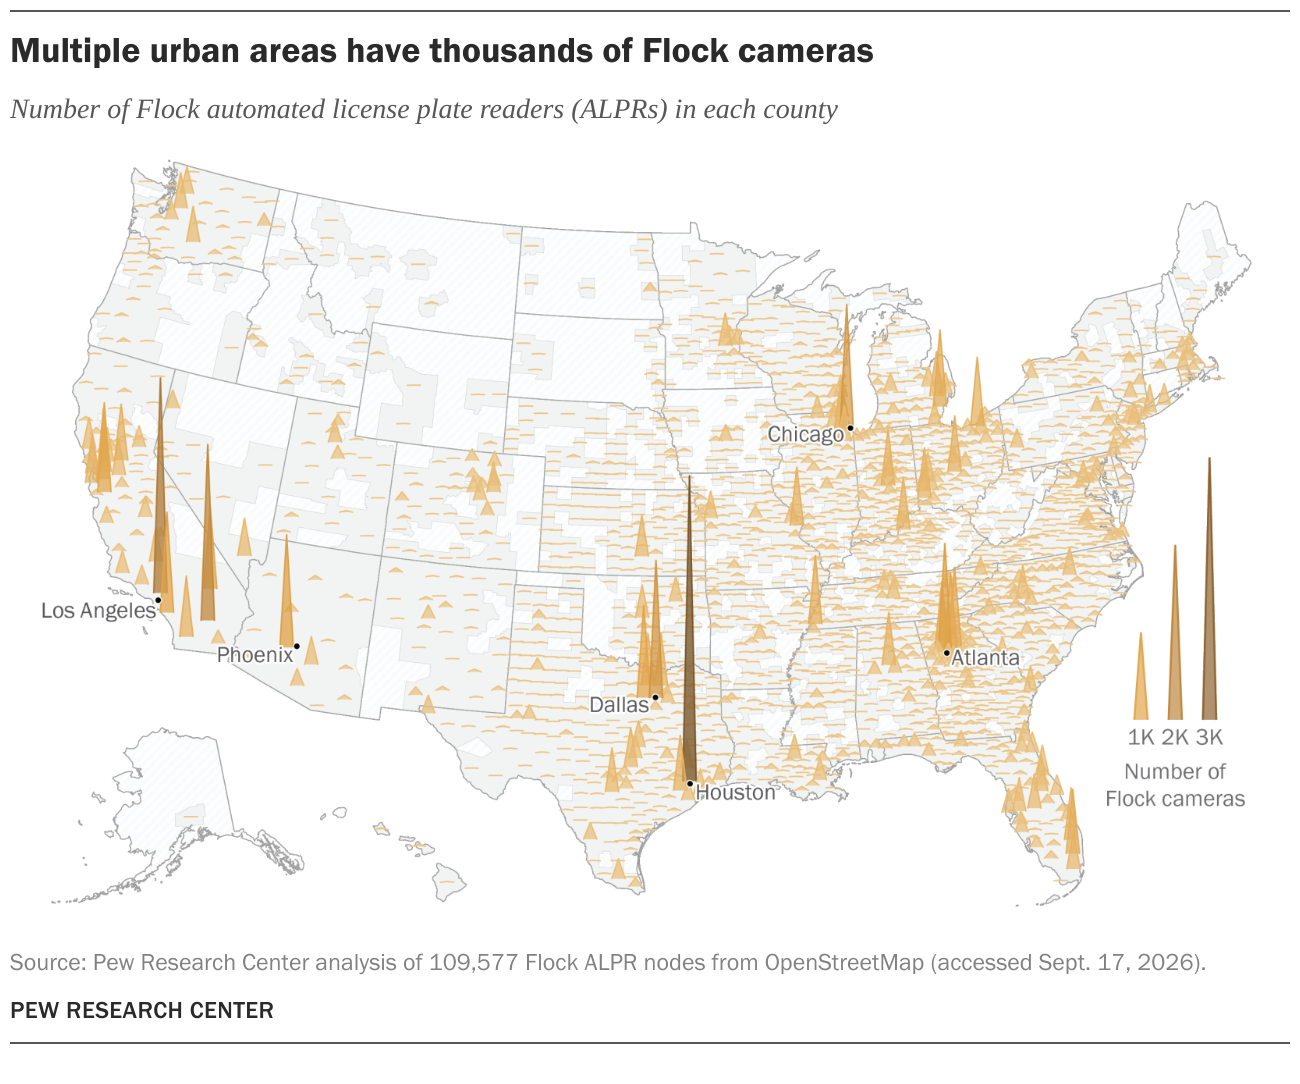
\includegraphics[width=0.85\textwidth]{flock-cameras.png}
\end{center}

This is a visualization I saw from Pew Research (link: \url{https://www.pewresearch.org/short-reads/2026/11/09/what-we-know-and-dont-know-about-flocks-license-plate-cameras/}). I thought it did a nice job showing that Flock Cameras tend to be concentrated in urban areas, since most of the big spikes are labeled with cities. Also, the spike is a nice way to leverage area/location, since a heat map would make it more difficult to see some of the differences - the spikes remind me of some of the maps with blue/red arrows from the midterm elections.

\vspace{0.5em}
I wish I could see a bar graph of the same data with a county-by-county breakdown, because it's still difficult to compare Atlanta and Chicago, for example. I am also curious about ``flock cameras per capita,'' i.e.\ adjusting for population in each county (I think one of the group projects is looking at this). So a bar graph with the top ten counties in terms of \texttt{(flock cameras / total population)} would be interesting. Also there are multiple spikes near Atlanta which I would want to see broken out.

\end{document}
